\section{Trådløs kommunikation}
Den trådløse kommunikation er designet til direkte kommunikation mellem mikrokontrolleren og NXT'en til styring af exoskelettet. Dertil skal der yderligere etablers en trådløs kommunikation til en computer til debugging, test af mikrokontrolleren samt datavisualisering.   

\noindent
Til implementeringen af den trådløse kommunikation afviges der fra det oprindelige design. Dette er som følge af opsætningen af bluetooth kommunikationen i mikrokontrolleren har fremkommet mere kompliceret end først antaget. Dette omfatter at der kræves en forståelse for diverse bluetooth programmeringsbiblioteker, samt relaterede funktioner til at programmere buletooth kommunikation. Tiden krævet til at implementere dette ville således blive for lang, og for usikker i forhold til endelig funktionalitet. Deril vælges der at implementere et mere simpelt og anvendeligt alternativ, bestående af to PSoC 4 M-Series Prototyping Kit board, der ses af \autoref{fig:PSoC_4200}

\begin{figure}[H]
	\centering
	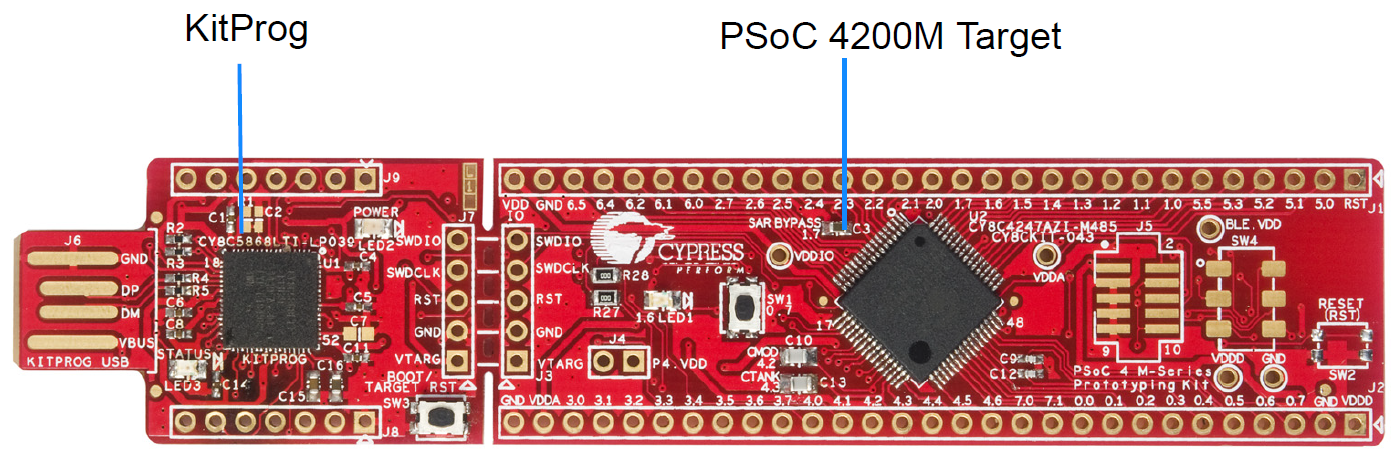
\includegraphics[width=1\textwidth]{figures/PSoC_4200_opdelt}
	\caption{CY8CKIT-043 PSoC 4 M-Series Prototyping Kit\citep{cypress42015}.}
	\label{fig:PSoC_4200}
\end{figure}

Dette board består af en KitProg og en PSoC 4200M enhed. KitProgen anvendes til at debugge og programmere koden, og PSoc 4200M er processoren hvorpå koden eksekveres. Yderligere er boardet udstyret med et EZ-BLE modul, der tillader trådløs kommunikation. 
Den ene PSoC 4200M tilkobles mikrokontrollern via UART forbindelse, og den anden tilsluttes computeren via USB og erstatter BLE donglen fra det oprindelige dessign. En illustation af hvordan kommunikationen transmiteres i det implementeret system ses af \autoref{fig:Traadloes_Komm_Imp}.

\begin{figure}[H]
	\centering
	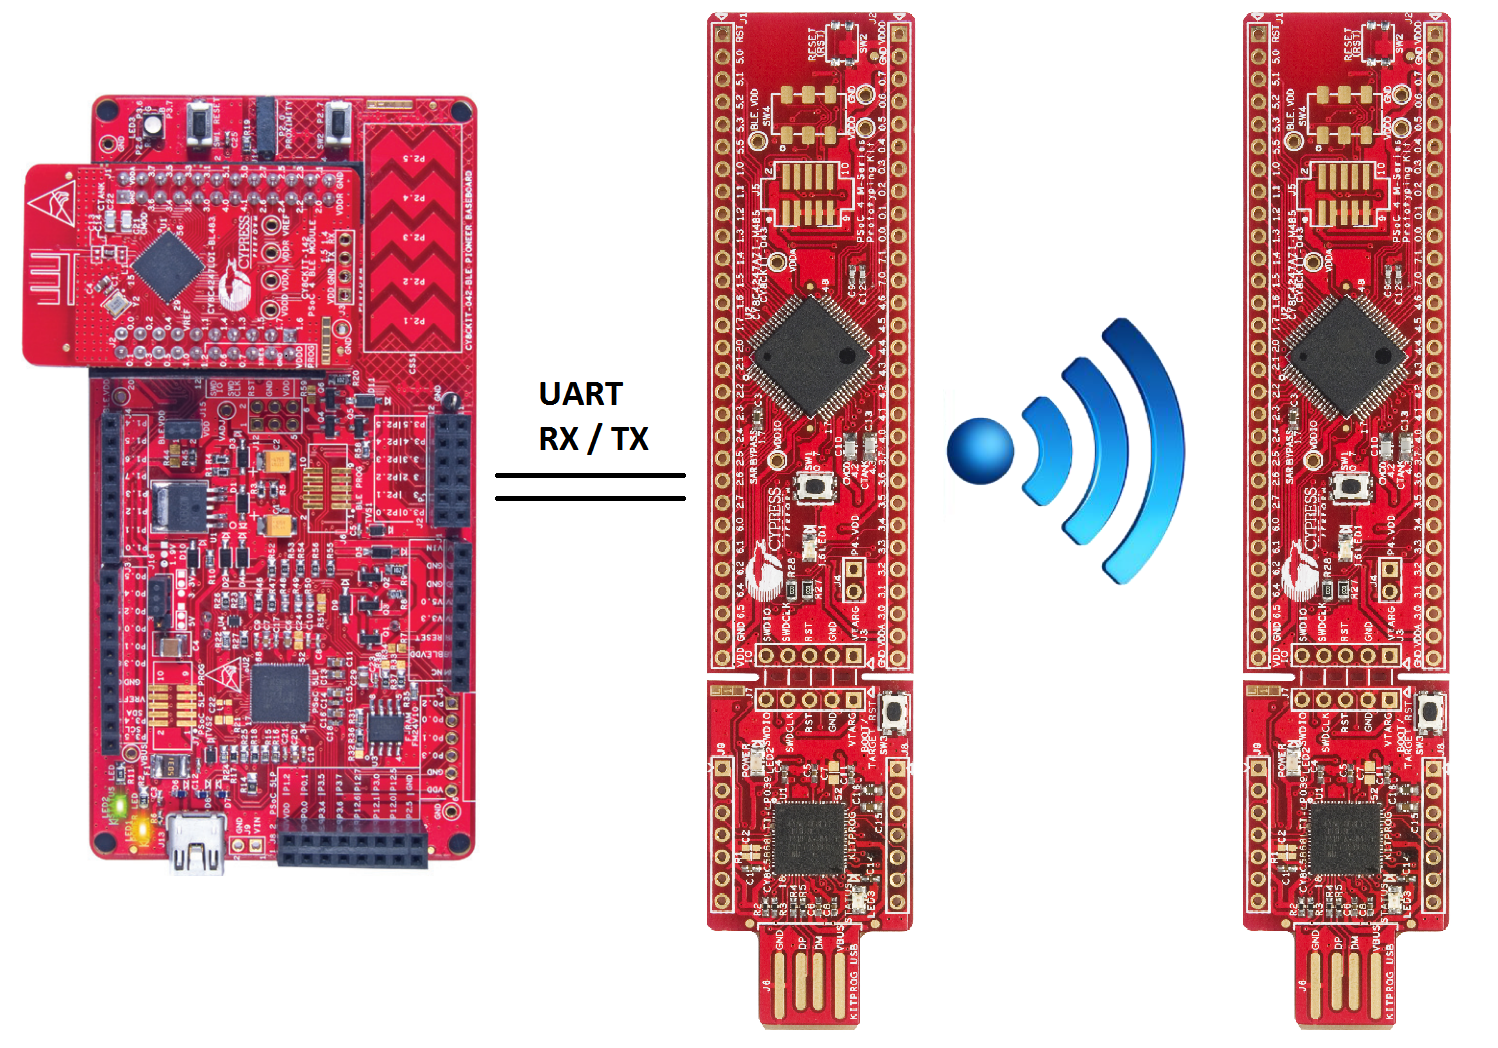
\includegraphics[width=1\textwidth]{figures/Traadloes_Komm_Imp}
	\caption{Illustration af kommunikation mellem mikrokontroller og computer.} 
	\label{fig:Traadloes_Komm_Imp}
\end{figure}

Begge PSoC 4200M enheder programmeres til at videregive information der modtages via BLE eller UART. Det ene EZ-BLE modul programmeres til central og det andet til periphiral.    